% Options for packages loaded elsewhere
\PassOptionsToPackage{unicode}{hyperref}
\PassOptionsToPackage{hyphens}{url}
%
\documentclass[
  12pt,
  a4paper,
  DIV=11,
  numbers=noendperiod]{scrreprt}

\usepackage{amsmath,amssymb}
\usepackage{setspace}
\usepackage{iftex}
\ifPDFTeX
  \usepackage[T1]{fontenc}
  \usepackage[utf8]{inputenc}
  \usepackage{textcomp} % provide euro and other symbols
\else % if luatex or xetex
  \usepackage{unicode-math}
  \defaultfontfeatures{Scale=MatchLowercase}
  \defaultfontfeatures[\rmfamily]{Ligatures=TeX,Scale=1}
\fi
\usepackage{lmodern}
\ifPDFTeX\else  
    % xetex/luatex font selection
\fi
% Use upquote if available, for straight quotes in verbatim environments
\IfFileExists{upquote.sty}{\usepackage{upquote}}{}
\IfFileExists{microtype.sty}{% use microtype if available
  \usepackage[]{microtype}
  \UseMicrotypeSet[protrusion]{basicmath} % disable protrusion for tt fonts
}{}
\usepackage{xcolor}
\usepackage{svg}
\setlength{\emergencystretch}{3em} % prevent overfull lines
\setcounter{secnumdepth}{5}
% Make \paragraph and \subparagraph free-standing
\ifx\paragraph\undefined\else
  \let\oldparagraph\paragraph
  \renewcommand{\paragraph}[1]{\oldparagraph{#1}\mbox{}}
\fi
\ifx\subparagraph\undefined\else
  \let\oldsubparagraph\subparagraph
  \renewcommand{\subparagraph}[1]{\oldsubparagraph{#1}\mbox{}}
\fi

\usepackage{color}
\usepackage{fancyvrb}
\newcommand{\VerbBar}{|}
\newcommand{\VERB}{\Verb[commandchars=\\\{\}]}
\DefineVerbatimEnvironment{Highlighting}{Verbatim}{commandchars=\\\{\}}
% Add ',fontsize=\small' for more characters per line
\usepackage{framed}
\definecolor{shadecolor}{RGB}{241,243,245}
\newenvironment{Shaded}{\begin{snugshade}}{\end{snugshade}}
\newcommand{\AlertTok}[1]{\textcolor[rgb]{0.68,0.00,0.00}{#1}}
\newcommand{\AnnotationTok}[1]{\textcolor[rgb]{0.37,0.37,0.37}{#1}}
\newcommand{\AttributeTok}[1]{\textcolor[rgb]{0.40,0.45,0.13}{#1}}
\newcommand{\BaseNTok}[1]{\textcolor[rgb]{0.68,0.00,0.00}{#1}}
\newcommand{\BuiltInTok}[1]{\textcolor[rgb]{0.00,0.23,0.31}{#1}}
\newcommand{\CharTok}[1]{\textcolor[rgb]{0.13,0.47,0.30}{#1}}
\newcommand{\CommentTok}[1]{\textcolor[rgb]{0.37,0.37,0.37}{#1}}
\newcommand{\CommentVarTok}[1]{\textcolor[rgb]{0.37,0.37,0.37}{\textit{#1}}}
\newcommand{\ConstantTok}[1]{\textcolor[rgb]{0.56,0.35,0.01}{#1}}
\newcommand{\ControlFlowTok}[1]{\textcolor[rgb]{0.00,0.23,0.31}{#1}}
\newcommand{\DataTypeTok}[1]{\textcolor[rgb]{0.68,0.00,0.00}{#1}}
\newcommand{\DecValTok}[1]{\textcolor[rgb]{0.68,0.00,0.00}{#1}}
\newcommand{\DocumentationTok}[1]{\textcolor[rgb]{0.37,0.37,0.37}{\textit{#1}}}
\newcommand{\ErrorTok}[1]{\textcolor[rgb]{0.68,0.00,0.00}{#1}}
\newcommand{\ExtensionTok}[1]{\textcolor[rgb]{0.00,0.23,0.31}{#1}}
\newcommand{\FloatTok}[1]{\textcolor[rgb]{0.68,0.00,0.00}{#1}}
\newcommand{\FunctionTok}[1]{\textcolor[rgb]{0.28,0.35,0.67}{#1}}
\newcommand{\ImportTok}[1]{\textcolor[rgb]{0.00,0.46,0.62}{#1}}
\newcommand{\InformationTok}[1]{\textcolor[rgb]{0.37,0.37,0.37}{#1}}
\newcommand{\KeywordTok}[1]{\textcolor[rgb]{0.00,0.23,0.31}{#1}}
\newcommand{\NormalTok}[1]{\textcolor[rgb]{0.00,0.23,0.31}{#1}}
\newcommand{\OperatorTok}[1]{\textcolor[rgb]{0.37,0.37,0.37}{#1}}
\newcommand{\OtherTok}[1]{\textcolor[rgb]{0.00,0.23,0.31}{#1}}
\newcommand{\PreprocessorTok}[1]{\textcolor[rgb]{0.68,0.00,0.00}{#1}}
\newcommand{\RegionMarkerTok}[1]{\textcolor[rgb]{0.00,0.23,0.31}{#1}}
\newcommand{\SpecialCharTok}[1]{\textcolor[rgb]{0.37,0.37,0.37}{#1}}
\newcommand{\SpecialStringTok}[1]{\textcolor[rgb]{0.13,0.47,0.30}{#1}}
\newcommand{\StringTok}[1]{\textcolor[rgb]{0.13,0.47,0.30}{#1}}
\newcommand{\VariableTok}[1]{\textcolor[rgb]{0.07,0.07,0.07}{#1}}
\newcommand{\VerbatimStringTok}[1]{\textcolor[rgb]{0.13,0.47,0.30}{#1}}
\newcommand{\WarningTok}[1]{\textcolor[rgb]{0.37,0.37,0.37}{\textit{#1}}}

\providecommand{\tightlist}{%
  \setlength{\itemsep}{0pt}\setlength{\parskip}{0pt}}\usepackage{longtable,booktabs,array}
\usepackage{calc} % for calculating minipage widths
% Correct order of tables after \paragraph or \subparagraph
\usepackage{etoolbox}
\makeatletter
\patchcmd\longtable{\par}{\if@noskipsec\mbox{}\fi\par}{}{}
\makeatother
% Allow footnotes in longtable head/foot
\IfFileExists{footnotehyper.sty}{\usepackage{footnotehyper}}{\usepackage{footnote}}
\makesavenoteenv{longtable}
\usepackage{graphicx}
\makeatletter
\def\maxwidth{\ifdim\Gin@nat@width>\linewidth\linewidth\else\Gin@nat@width\fi}
\def\maxheight{\ifdim\Gin@nat@height>\textheight\textheight\else\Gin@nat@height\fi}
\makeatother
% Scale images if necessary, so that they will not overflow the page
% margins by default, and it is still possible to overwrite the defaults
% using explicit options in \includegraphics[width, height, ...]{}
\setkeys{Gin}{width=\maxwidth,height=\maxheight,keepaspectratio}
% Set default figure placement to htbp
\makeatletter
\def\fps@figure{htbp}
\makeatother

\usepackage{indentfirst}
\usepackage{float}
\floatplacement{figure}{H}
\IfFileExists{plex-otf.sty}{
  %% Full TeXlive
  \usepackage[
    % math,
    RM={Scale=0.94},SS={Scale=0.94},SScon={Scale=0.94},TT={Scale=MatchLowercase,FakeStretch=0.9},
    DefaultFeatures={Ligatures=Common}
  ]{plex-otf}
  % \usepackage[Scale=MatchUppercase]{juliamono}
}{
  %% TinyTeX
  \usepackage{libertine}
}
\KOMAoption{captions}{tableheading}
\makeatletter
\@ifpackageloaded{caption}{}{\usepackage{caption}}
\AtBeginDocument{%
\ifdefined\contentsname
  \renewcommand*\contentsname{Содержание}
\else
  \newcommand\contentsname{Содержание}
\fi
\ifdefined\listfigurename
  \renewcommand*\listfigurename{Список иллюстраций}
\else
  \newcommand\listfigurename{Список иллюстраций}
\fi
\ifdefined\listtablename
  \renewcommand*\listtablename{Список таблиц}
\else
  \newcommand\listtablename{Список таблиц}
\fi
\ifdefined\figurename
  \renewcommand*\figurename{Рисунок}
\else
  \newcommand\figurename{Рисунок}
\fi
\ifdefined\tablename
  \renewcommand*\tablename{Таблица}
\else
  \newcommand\tablename{Таблица}
\fi
}
\@ifpackageloaded{float}{}{\usepackage{float}}
\floatstyle{ruled}
\@ifundefined{c@chapter}{\newfloat{codelisting}{h}{lop}}{\newfloat{codelisting}{h}{lop}[chapter]}
\floatname{codelisting}{Список}
\newcommand*\listoflistings{\listof{codelisting}{Листинги}}
\makeatother
\makeatletter
\makeatother
\makeatletter
\@ifpackageloaded{caption}{}{\usepackage{caption}}
\@ifpackageloaded{subcaption}{}{\usepackage{subcaption}}
\makeatother
\ifLuaTeX
\usepackage[bidi=basic]{babel}
\else
\usepackage[bidi=default]{babel}
\fi
\babelprovide[main,import]{russian}
\babelprovide[import]{english}
% get rid of language-specific shorthands (see #6817):
\let\LanguageShortHands\languageshorthands
\def\languageshorthands#1{}
\ifLuaTeX
  \usepackage{selnolig}  % disable illegal ligatures
\fi
\usepackage[style=gost-numeric,backend=biber,langhook=extras,autolang=other*]{biblatex}
\addbibresource{bib/cite.bib}
\usepackage{csquotes}
\usepackage{bookmark}

\IfFileExists{xurl.sty}{\usepackage{xurl}}{} % add URL line breaks if available
\urlstyle{same} % disable monospaced font for URLs
\hypersetup{
  pdftitle={Отчёта по лабораторной работе 8},
  pdfauthor={Нджову Нелиа},
  pdflang={ru-RU},
  hidelinks,
  pdfcreator={LaTeX via pandoc}}

\title{Отчёта по лабораторной работе 8}
\usepackage{etoolbox}
\makeatletter
\providecommand{\subtitle}[1]{% add subtitle to \maketitle
  \apptocmd{\@title}{\par {\large #1 \par}}{}{}
}
\makeatother
\subtitle{Иммитационное моделирование}
\author{Нджову Нелиа}
\date{}

\begin{document}
\maketitle

\renewcommand*\contentsname{Содержание}
{
\setcounter{tocdepth}{1}
\tableofcontents
}
\listoffigures
\listoftables
\setstretch{1.5}
\chapter{Цель
работы}\label{ux446ux435ux43bux44c-ux440ux430ux431ux43eux442ux44b}

Цель этой лабораторной работы - Изучить дискретно-событийный подход к
имитационному моделированию на примере классической модели
распространения инфекции SIR. Реализовать стохастическую
дискретно-событийную модель в виде программного комплекса на языке
Julia. Провести анализ влияния параметров, сравнить со стохастической и
детерминированной версиями, оценить производительность и модифицировать
модель.

\chapter{Задание}\label{ux437ux430ux434ux430ux43dux438ux435}

\begin{enumerate}
\def\labelenumi{\arabic{enumi}.}
\item
  Структура программы
\item
  Скрипт запуска
\item
  Анализ чувствительности к параметрам
\item
  Детерминированная длительность болезни
\item
  Оценка производительности
\item
  Сохранение результатов в CSV
\item
  Добавление демографических событий
\item
  Вакцинация
\item
  Модель SEIR
\end{enumerate}

\chapter{Теоретическое
введение}\label{ux442ux435ux43eux440ux435ux442ux438ux447ux435ux441ux43aux43eux435-ux432ux432ux435ux434ux435ux43dux438ux435}

Модель SIR - это фундаментальная сегментарная модель в эпидемиологии,
которая описывает распространение инфекционного заболевания в замкнутой
популяции.

Модель делит все население (N) на три отдельные, взаимоисключающие
группы:

\begin{itemize}
\item
  S (Восприимчивые): люди, которые здоровы, но могут заразиться.
\item
  I (Инфекционные): люди, которые в настоящее время больны и могут
  передать болезнь восприимчивым людям.
\item
  R (выздоровевшие): люди, которые выздоровели (и считаются
  невосприимчивыми) или умерли. Они больше не участвуют в процессе
  передачи.
\end{itemize}

Общая численность населения постоянна: N=S+I+R.

\chapter{Выполнение лабораторной
работы}\label{ux432ux44bux43fux43eux43bux43dux435ux43dux438ux435-ux43bux430ux431ux43eux440ux430ux442ux43eux440ux43dux43eux439-ux440ux430ux431ux43eux442ux44b}

\section{1. Структура
программы}\label{ux441ux442ux440ux443ux43aux442ux443ux440ux430-ux43fux440ux43eux433ux440ux430ux43cux43cux44b}

Я создала файл src/Sir\_model.jl и скопировала заданный скрипт в него.
Скрипт реализует ядро модели SIR с дискретными событиями. Он определяет
структуры данных, логику поведения агентов и функции управления
симуляцией(рис.1)

\begin{figure}

\centering{


\includegraphics[width=0.7\textwidth,height=\textheight]{image/pic1.png}

}

\caption{\label{fig-001}Структура программы}

\end{figure}%

Я запускала код и все хорошо сработал.

\section{2. Скрипт
запуска}\label{ux441ux43aux440ux438ux43fux442-ux437ux430ux43fux443ux441ux43aux430}

Я создала файл scripts/sir\_des.jl и скопировала заданный скрипт в него.
Этот скрипт загружает ядро sir\_model.jl, устанавливает параметры
моделирования, запускает моделирование SIR с дискретными событиями и
генерирует график динамики S, I и R с течением времени.(рис.2)

\begin{figure}

\centering{


\includegraphics[width=0.7\textwidth,height=\textheight]{image/pic2.png}

}

\caption{\label{fig-002}Скрипт запуска}

\end{figure}%

Я запускала код и все хорошо сработал, получила график ниже(рис.3)

\begin{figure}

\centering{

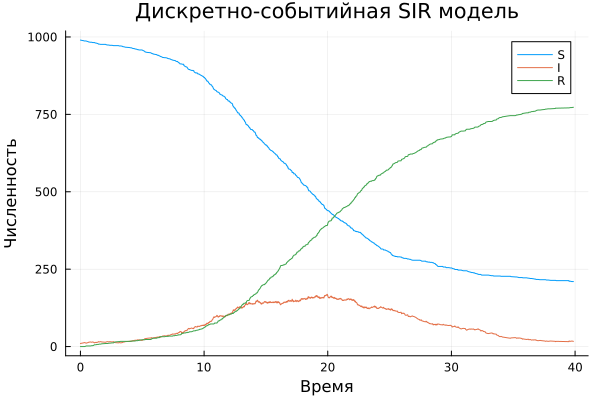
\includegraphics[width=0.7\textwidth,height=\textheight]{image/sir_des.png}

}

\caption{\label{fig-003}График}

\end{figure}%

\textbf{Ниже приведен код, результаты расчетов и графики для кода в
файле scripts/sir\_des.qmd}

\section{Модель SIR}\label{ux43cux43eux434ux435ux43bux44c-sir}

Модель создается, процессы активируются, и запуск выполняется. Результат
преобразуется во фрейм данных. График с кривыми S, I, R создается и
сохраняется

\begin{Shaded}
\begin{Highlighting}[]
\ImportTok{using} \BuiltInTok{DrWatson}
\PreprocessorTok{@quickactivate} \StringTok{"project"}
\FunctionTok{include}\NormalTok{(}\FunctionTok{srcdir}\NormalTok{(}\StringTok{"Sir\_model.jl"}\NormalTok{))}
\ImportTok{using} \BuiltInTok{Random}\NormalTok{, }\BuiltInTok{StatsPlots}\NormalTok{, }\BuiltInTok{BenchmarkTools}\NormalTok{, }\BuiltInTok{CSV}\NormalTok{, }\BuiltInTok{Dates}
\FunctionTok{gr}\NormalTok{(fmt}\OperatorTok{=:}\NormalTok{png)}
\end{Highlighting}
\end{Shaded}

\begin{verbatim}
┌ Warning: DrWatson could not find find a project file by recursively checking given `dir` and its parents. Returning `nothing` instead.
│ (given dir: /home/nelianjovu)
└ @ DrWatson ~/.julia/packages/DrWatson/2QF5p/src/project_setup.jl:84
\end{verbatim}

\begin{verbatim}
Plots.GRBackend()
\end{verbatim}

Параметры модели

\begin{Shaded}
\begin{Highlighting}[]
\NormalTok{tmax }\OperatorTok{=} \FloatTok{40.0}
\NormalTok{u0 }\OperatorTok{=}\NormalTok{ [}\FloatTok{990}\NormalTok{, }\FloatTok{10}\NormalTok{, }\FloatTok{0}\NormalTok{] }\CommentTok{\# S, I, R}
\NormalTok{p }\OperatorTok{=}\NormalTok{ [}\FloatTok{0.05}\NormalTok{, }\FloatTok{10.0}\NormalTok{, }\FloatTok{0.25}\NormalTok{] }\CommentTok{\# β, c, γ}

\BuiltInTok{Random}\NormalTok{.}\FunctionTok{seed!}\NormalTok{(}\FloatTok{1234}\NormalTok{)}
\end{Highlighting}
\end{Shaded}

\begin{verbatim}
TaskLocalRNG()
\end{verbatim}

Запуск модели

\begin{Shaded}
\begin{Highlighting}[]
\NormalTok{des\_model }\OperatorTok{=} \FunctionTok{MakeSIRModel}\NormalTok{(u0, p)}
\FunctionTok{activate}\NormalTok{(des\_model)}
\FunctionTok{sir\_run}\NormalTok{(des\_model, tmax)}
\NormalTok{data\_des }\OperatorTok{=} \FunctionTok{out}\NormalTok{(des\_model)}
\end{Highlighting}
\end{Shaded}

\begin{tabular}{r|cccc}
    & t & S & I & R\\
    \hline
    & Float64 & Int64 & Int64 & Int64\\
    \hline
    1 & 0.0 & 990 & 10 & 0 \\
    2 & 0.110851 & 989 & 11 & 0 \\
    3 & 0.249585 & 988 & 12 & 0 \\
    4 & 0.314392 & 987 & 13 & 0 \\
    5 & 0.418738 & 987 & 12 & 1 \\
    6 & 0.457041 & 987 & 11 & 2 \\
    7 & 0.528895 & 986 & 12 & 2 \\
    8 & 0.619502 & 985 & 13 & 2 \\
    9 & 0.657704 & 984 & 14 & 2 \\
    10 & 0.807485 & 983 & 15 & 2 \\
    11 & 0.913646 & 983 & 14 & 3 \\
    12 & 0.976249 & 982 & 15 & 3 \\
    13 & 1.07816 & 982 & 14 & 4 \\
    14 & 1.09161 & 982 & 13 & 5 \\
    15 & 1.1487 & 982 & 12 & 6 \\
    16 & 1.17259 & 981 & 13 & 6 \\
    17 & 1.2789 & 980 & 14 & 6 \\
    18 & 1.30828 & 980 & 13 & 7 \\
    19 & 1.37686 & 979 & 14 & 7 \\
    20 & 1.44574 & 978 & 15 & 7 \\
    21 & 1.45046 & 977 & 16 & 7 \\
    22 & 1.51802 & 977 & 15 & 8 \\
    23 & 1.63961 & 976 & 16 & 8 \\
    24 & 1.71622 & 976 & 15 & 9 \\
    25 & 2.05024 & 976 & 14 & 10 \\
    26 & 2.0729 & 975 & 15 & 10 \\
    27 & 2.20607 & 974 & 16 & 10 \\
    28 & 2.30437 & 974 & 15 & 11 \\
    29 & 2.37251 & 973 & 16 & 11 \\
    30 & 2.56655 & 973 & 15 & 12 \\
    $\dots$ & $\dots$ & $\dots$ & $\dots$ & $\dots$ \\
\end{tabular}

Визуализация

\begin{Shaded}
\begin{Highlighting}[]
\PreprocessorTok{@df}\NormalTok{ data\_des }\FunctionTok{plot}\NormalTok{(}
    \OperatorTok{:}\NormalTok{t,}
\NormalTok{    [}\OperatorTok{:}\NormalTok{S }\OperatorTok{:}\NormalTok{I }\OperatorTok{:}\NormalTok{R],}
\NormalTok{    labels }\OperatorTok{=}\NormalTok{ [}\StringTok{"S"} \StringTok{"I"} \StringTok{"R"}\NormalTok{],}
\NormalTok{    xlab }\OperatorTok{=} \StringTok{"Время"}\NormalTok{,}
\NormalTok{    ylab }\OperatorTok{=} \StringTok{"Численность"}\NormalTok{,}
\NormalTok{    title }\OperatorTok{=} \StringTok{"Дискретно{-}событийная SIR модель"}\NormalTok{,}
\NormalTok{)}
\FunctionTok{savefig}\NormalTok{(}\FunctionTok{plotsdir}\NormalTok{(}\StringTok{"sir\_des.png"}\NormalTok{))}

\NormalTok{filename }\OperatorTok{=} \StringTok{"sir\_}\SpecialCharTok{$}\NormalTok{(u0[}\FloatTok{1}\NormalTok{])}\StringTok{\_}\SpecialCharTok{$}\NormalTok{(u0[}\FloatTok{2}\NormalTok{])}\StringTok{\_}\SpecialCharTok{$}\NormalTok{(p[}\FloatTok{1}\NormalTok{])}\StringTok{\_}\SpecialCharTok{$}\NormalTok{(p[}\FloatTok{2}\NormalTok{])}\StringTok{\_}\SpecialCharTok{$}\NormalTok{(p[}\FloatTok{3}\NormalTok{])}\StringTok{.csv"}
\NormalTok{CSV.}\FunctionTok{write}\NormalTok{(}\FunctionTok{datadir}\NormalTok{(}\StringTok{"sims"}\NormalTok{, filename), data\_des)}
\end{Highlighting}
\end{Shaded}

\begin{verbatim}
"/home/nelianjovu/work/study/2026-1/2026-1==study--simulationmod/2026-1--study--simulationmod/labs/lab08/project/data/sims/sir_990_10_0.05_10.0_0.25.csv"
\end{verbatim}

\section{3. Анализ чувствительности к
параметрам}\label{ux430ux43dux430ux43bux438ux437-ux447ux443ux432ux441ux442ux432ux438ux442ux435ux43bux44cux43dux43eux441ux442ux438-ux43a-ux43fux430ux440ux430ux43cux435ux442ux440ux430ux43c}

Я создала файл scripts/sensitivity\_beta.jl, в него, я писала код,
похоже с заданный скрипт но с разными значениями \(\beta\) - вероятность
передачи инфекции при одном контакте между заразным и восприимчивым
(безразмерная величина, от 0 до 1). Я проанализировала пик заражения,
время пика и конечное количество выздоровевших людей для каждого
значения \(\beta\)

По мере того, как \(\beta\) увеличивает пик заражения, число
выздоровевших увеличивается, а время пика уменьшается(рис.4)

\begin{figure}

\centering{


\includegraphics[width=0.7\textwidth,height=\textheight]{image/pic3.png}

}

\caption{\label{fig-003}Анализ разных параметрах \(\beta\)}

\end{figure}%

Я создала файл scripts/sensitivity\_c.jl, в него, я писала код, похоже с
заданный скрипт но с разными значениями c - среднее число контактов
(достаточно тесных для передачи инфекции) одного человека в единицу
времени. Я проанализировала пик заражения, время пика и конечное
количество выздоровевших людей для каждого значения c

По мере того, как c увеличивает, пик заражения и число выздоровевших
увеличивается, а время пика уменьшается(рис.5)

\begin{figure}

\centering{


\includegraphics[width=0.7\textwidth,height=\textheight]{image/pic5.png}

}

\caption{\label{fig-003}Анализ разных параметрах c}

\end{figure}%

Я создала файл scripts/sensitivity\_gamma.jl, в него, я писала код,
похоже с заданный скрипт но с разными значениями \(\gamma\) - скорость
выздоровления (доля инфицированных, выздоравливающих в единицу времени).
Я проанализировала пик заражения, время пика и конечное количество
выздоровевших людей для каждого значения \(\gamma\)

По мере того, как \(\gamma\) увеличивает, пик заражения и число
выздоровевших уменьшается, а время пика, сначала увеличивается а потом
уменьшается(рис.6)

\begin{figure}

\centering{


\includegraphics[width=0.7\textwidth,height=\textheight]{image/pic6.png}

}

\caption{\label{fig-003}Анализ разных параметрах \(\gamma\)}

\end{figure}%

\section{4. Детерминированная длительность
болезни}\label{ux434ux435ux442ux435ux440ux43cux438ux43dux438ux440ux43eux432ux430ux43dux43dux430ux44f-ux434ux43bux438ux442ux435ux43bux44cux43dux43eux441ux442ux44c-ux431ux43eux43bux435ux437ux43dux438}

Я заменяю экспоненциальное время восстановления на фиксированное
значение 1/γ(рис.7)

\begin{figure}

\centering{


\includegraphics[width=0.7\textwidth,height=\textheight]{image/pic7.png}

}

\caption{\label{fig-003}фиксированное значение 1/γ}

\end{figure}%

Я сравниваю детерминированную версию со стохастической версией. Что
касается стохастической модели, то мы можем видеть, что она немного
грубовата, поскольку отражает реальность происходящего. Что касается
детерминированной модели, то она немного сглажена, поскольку показывает
вычислительную модель, основанную на средних значениях и
уравнениях.(рис.8)

\begin{figure}

\centering{

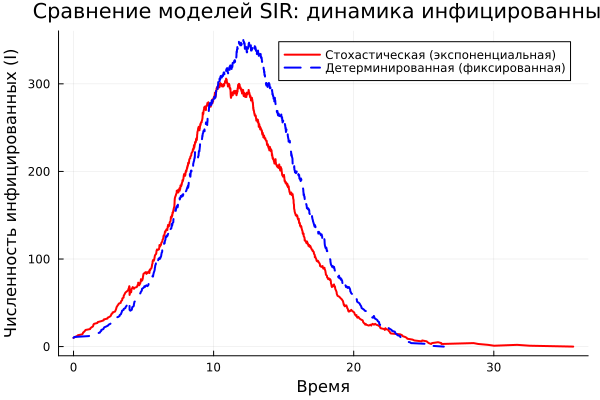
\includegraphics[width=0.7\textwidth,height=\textheight]{image/sir_comparison.png}

}

\caption{\label{fig-003}Сравнение версии}

\end{figure}%

\textbf{Ниже приведен код, результаты расчетов и графики для кода в
файле scripts/sir\_deterministic.qmd}

\section{Модель SIR}\label{ux43cux43eux434ux435ux43bux44c-sir-1}

Модель создается, процессы активируются, и запуск выполняется. Результат
преобразуется во фрейм данных. График с кривыми S, I, R создается и
сохраняется

\begin{Shaded}
\begin{Highlighting}[]
\ImportTok{using} \BuiltInTok{DrWatson}
\PreprocessorTok{@quickactivate} \StringTok{"project"}
\FunctionTok{include}\NormalTok{(}\FunctionTok{srcdir}\NormalTok{(}\StringTok{"Sir\_model.jl"}\NormalTok{))}
\FunctionTok{include}\NormalTok{(}\FunctionTok{srcdir}\NormalTok{(}\StringTok{"Sir\_deterministic.jl"}\NormalTok{))}
\ImportTok{using} \BuiltInTok{Random}\NormalTok{, }\BuiltInTok{StatsPlots}\NormalTok{, }\BuiltInTok{BenchmarkTools}
\FunctionTok{gr}\NormalTok{(fmt}\OperatorTok{=:}\NormalTok{png)}
\end{Highlighting}
\end{Shaded}

\begin{verbatim}
┌ Warning: DrWatson could not find find a project file by recursively checking given `dir` and its parents. Returning `nothing` instead.
│ (given dir: /home/nelianjovu)
└ @ DrWatson ~/.julia/packages/DrWatson/2QF5p/src/project_setup.jl:84
\end{verbatim}

\begin{verbatim}
Plots.GRBackend()
\end{verbatim}

Параметры модели

\begin{Shaded}
\begin{Highlighting}[]
\NormalTok{tmax }\OperatorTok{=} \FloatTok{40.0}
\NormalTok{u0 }\OperatorTok{=}\NormalTok{ [}\FloatTok{990}\NormalTok{, }\FloatTok{10}\NormalTok{, }\FloatTok{0}\NormalTok{] }\CommentTok{\# S, I, R}
\NormalTok{p }\OperatorTok{=}\NormalTok{ [}\FloatTok{0.05}\NormalTok{, }\FloatTok{10.0}\NormalTok{, }\FloatTok{0.25}\NormalTok{] }\CommentTok{\# β, c, γ}

\BuiltInTok{Random}\NormalTok{.}\FunctionTok{seed!}\NormalTok{(}\FloatTok{1234}\NormalTok{)}
\end{Highlighting}
\end{Shaded}

\begin{verbatim}
TaskLocalRNG()
\end{verbatim}

Запуск модели

\begin{Shaded}
\begin{Highlighting}[]
\NormalTok{stoch\_model }\OperatorTok{=} \FunctionTok{MakeSIRModelD}\NormalTok{(u0, p)}
\FunctionTok{activate}\NormalTok{(stoch\_model)}
\FunctionTok{sir\_run}\NormalTok{(stoch\_model, tmax)}
\NormalTok{data\_stoch }\OperatorTok{=} \FunctionTok{out}\NormalTok{(stoch\_model)}

\NormalTok{deter\_model }\OperatorTok{=} \FunctionTok{MakeSIRModelD}\NormalTok{(u0, p)}
\FunctionTok{activate}\NormalTok{(deter\_model)}
\FunctionTok{sir\_run}\NormalTok{(deter\_model, tmax)}
\NormalTok{data\_deter }\OperatorTok{=} \FunctionTok{out}\NormalTok{(deter\_model)}
\end{Highlighting}
\end{Shaded}

\begin{tabular}{r|cccc}
    & t & S & I & R\\
    \hline
    & Float64 & Int64 & Int64 & Int64\\
    \hline
    1 & 0.0 & 990 & 10 & 0 \\
    2 & 0.0550178 & 989 & 11 & 0 \\
    3 & 1.08959 & 988 & 12 & 0 \\
    4 & 1.27335 & 987 & 13 & 0 \\
    5 & 1.64664 & 986 & 14 & 0 \\
    6 & 1.67492 & 985 & 15 & 0 \\
    7 & 1.87887 & 984 & 16 & 0 \\
    8 & 1.90739 & 983 & 17 & 0 \\
    9 & 1.9808 & 982 & 18 & 0 \\
    10 & 1.98296 & 981 & 19 & 0 \\
    11 & 2.13035 & 980 & 20 & 0 \\
    12 & 2.1582 & 979 & 21 & 0 \\
    13 & 2.19511 & 978 & 22 & 0 \\
    14 & 2.34092 & 977 & 23 & 0 \\
    15 & 2.4615 & 976 & 24 & 0 \\
    16 & 2.50577 & 975 & 25 & 0 \\
    17 & 2.62611 & 974 & 26 & 0 \\
    18 & 2.68531 & 973 & 27 & 0 \\
    19 & 2.80709 & 972 & 28 & 0 \\
    20 & 2.83319 & 971 & 29 & 0 \\
    21 & 2.86673 & 970 & 30 & 0 \\
    22 & 3.02579 & 969 & 31 & 0 \\
    23 & 3.02821 & 968 & 32 & 0 \\
    24 & 3.03356 & 967 & 33 & 0 \\
    25 & 3.2002 & 966 & 34 & 0 \\
    26 & 3.28802 & 965 & 35 & 0 \\
    27 & 3.29785 & 964 & 36 & 0 \\
    28 & 3.38219 & 963 & 37 & 0 \\
    29 & 3.40548 & 962 & 38 & 0 \\
    30 & 3.42886 & 961 & 39 & 0 \\
    $\dots$ & $\dots$ & $\dots$ & $\dots$ & $\dots$ \\
\end{tabular}

Визуализация

\begin{Shaded}
\begin{Highlighting}[]
\NormalTok{plot1 }\OperatorTok{=} \PreprocessorTok{@df}\NormalTok{ data\_deter }\FunctionTok{plot}\NormalTok{(}
    \OperatorTok{:}\NormalTok{t,}
\NormalTok{    [}\OperatorTok{:}\NormalTok{S }\OperatorTok{:}\NormalTok{I }\OperatorTok{:}\NormalTok{R],}
\NormalTok{    labels }\OperatorTok{=}\NormalTok{ [}\StringTok{"S"} \StringTok{"I"} \StringTok{"R"}\NormalTok{],}
\NormalTok{    xlab }\OperatorTok{=} \StringTok{"Время"}\NormalTok{,}
\NormalTok{    ylab }\OperatorTok{=} \StringTok{"Численность"}\NormalTok{,}
\NormalTok{    title }\OperatorTok{=} \StringTok{"Детерминированная SIR модель (фиксированное выздоровление)"}\NormalTok{,}
\NormalTok{)}
\FunctionTok{savefig}\NormalTok{(}\FunctionTok{plotsdir}\NormalTok{(}\StringTok{"sir\_deter.png"}\NormalTok{))}
\FunctionTok{display}\NormalTok{(plot1)}

\NormalTok{plot2 }\OperatorTok{=} \PreprocessorTok{@df}\NormalTok{ data\_stoch }\FunctionTok{plot}\NormalTok{(}
    \OperatorTok{:}\NormalTok{t,}
\NormalTok{    [}\OperatorTok{:}\NormalTok{S }\OperatorTok{:}\NormalTok{I }\OperatorTok{:}\NormalTok{R],}
\NormalTok{    labels }\OperatorTok{=}\NormalTok{ [}\StringTok{"S"} \StringTok{"I"} \StringTok{"R"}\NormalTok{],}
\NormalTok{    xlab }\OperatorTok{=} \StringTok{"Время"}\NormalTok{,}
\NormalTok{    ylab }\OperatorTok{=} \StringTok{"Численность"}\NormalTok{,}
\NormalTok{    title }\OperatorTok{=} \StringTok{"Стохастическая SIR модель (экспоненциальное выздоровление)"}\NormalTok{,}
\NormalTok{)}
\FunctionTok{savefig}\NormalTok{(}\FunctionTok{plotsdir}\NormalTok{(}\StringTok{"sir\_stoch.png"}\NormalTok{))}
\FunctionTok{display}\NormalTok{(plot2)}

\NormalTok{plot3 }\OperatorTok{=} \FunctionTok{plot}\NormalTok{(}
\NormalTok{    data\_stoch.t, data\_stoch.I,}
\NormalTok{    label }\OperatorTok{=} \StringTok{"Стохастическая (экспоненциальная)"}\NormalTok{,}
\NormalTok{    xlabel }\OperatorTok{=} \StringTok{"Время"}\NormalTok{,}
\NormalTok{    ylabel }\OperatorTok{=} \StringTok{"Численность инфицированных (I)"}\NormalTok{,}
\NormalTok{    title }\OperatorTok{=} \StringTok{"Сравнение моделей SIR: динамика инфицированных"}\NormalTok{,}
\NormalTok{    linewidth }\OperatorTok{=} \FloatTok{2}\NormalTok{,}
\NormalTok{    color }\OperatorTok{=} \OperatorTok{:}\NormalTok{red,}
\NormalTok{    legend }\OperatorTok{=} \OperatorTok{:}\NormalTok{topright,}
\NormalTok{    grid }\OperatorTok{=} \ConstantTok{true}\NormalTok{,}
\NormalTok{)}
\FunctionTok{plot!}\NormalTok{(}
\NormalTok{    plot3,}
\NormalTok{    data\_deter.t, data\_deter.I,}
\NormalTok{    label }\OperatorTok{=} \StringTok{"Детерминированная (фиксированная)"}\NormalTok{,}
\NormalTok{    linewidth }\OperatorTok{=} \FloatTok{2}\NormalTok{,}
\NormalTok{    color }\OperatorTok{=} \OperatorTok{:}\NormalTok{blue,}
\NormalTok{)}
\FunctionTok{savefig}\NormalTok{(}\FunctionTok{plotsdir}\NormalTok{(}\StringTok{"sir\_comparison.png"}\NormalTok{))}
\end{Highlighting}
\end{Shaded}

\includesvg{simmod-lab08-report (Нджову Нелиа)_files/figure-pdf/cell-10-output-1.svg}

\includesvg{simmod-lab08-report (Нджову Нелиа)_files/figure-pdf/cell-10-output-2.svg}

\begin{verbatim}
"/home/nelianjovu/work/study/2026-1/2026-1==study--simulationmod/2026-1--study--simulationmod/labs/lab08/project/plots/sir_comparison.png"
\end{verbatim}

\section{5. Оценка
производительности}\label{ux43eux446ux435ux43dux43aux430-ux43fux440ux43eux438ux437ux432ux43eux434ux438ux442ux435ux43bux44cux43dux43eux441ux442ux438}

Используя макрос \textcite{benchmark}, я измеряю время выполнения
sir\_run для популяции из 10 000 человек(рис.9)

\begin{figure}

\centering{


\includegraphics[width=0.7\textwidth,height=\textheight]{image/pic9.png}

}

\caption{\label{fig-003}Измерение время выполнения программа}

\end{figure}%

Модель была протестирована на популяции из 10 000 особей в течение 40
единиц времени. Моделирование завершилось в среднем менее чем за 0,01
секунды, продемонстрировав, что реализация на основе ConcurrentSim
является высокоэффективной для популяций такого размера(рис.10)

\begin{figure}

\centering{


\includegraphics[width=0.7\textwidth,height=\textheight]{image/pic10.png}

}

\caption{\label{fig-003}Время выполнения программа}

\end{figure}%

\section{6. Сохранение результатов в
CSV}\label{ux441ux43eux445ux440ux430ux43dux435ux43dux438ux435-ux440ux435ux437ux443ux43bux44cux442ux430ux442ux43eux432-ux432-csv}

Я добавляю автоматическое сохранение итоговой таблицы в каталог
data/sims/ с уникальным именем, содержащим параметры запуска(рис.11)

\begin{figure}

\centering{


\includegraphics[width=0.7\textwidth,height=\textheight]{image/pic11.png}

}

\caption{\label{fig-003}сохранение итоговой таблицы}

\end{figure}%

Код сработал, и файл был сохранен(рис.12)

\begin{figure}

\centering{


\includegraphics[width=0.7\textwidth,height=\textheight]{image/pic12.png}

}

\caption{\label{fig-003}сохранение итоговой таблицы}

\end{figure}%

\section{7. Добавление демографических
событий}\label{ux434ux43eux431ux430ux432ux43bux435ux43dux438ux435-ux434ux435ux43cux43eux433ux440ux430ux444ux438ux447ux435ux441ux43aux438ux445-ux441ux43eux431ux44bux442ux438ux439}

Я расширяю модель, добавляя к жизненному циклу индивидуума возможность
смерти (с постоянной интенсивностью \(\mu\)) и рождения новых
восприимчивых особей. Смерть удаляет индивидуума из популяции, рождение
добавляет нового в состояние : S.(рис 13)

\begin{figure}

\centering{


\includegraphics[width=0.7\textwidth,height=\textheight]{image/pic14.png}

}

\caption{\label{fig-003}добавление возможности смерти и рождения}

\end{figure}%

В отличие от стандартной модели SIR, в модели с демографией количество
выздоровевших людей увеличивается, а затем снова начинает уменьшаться.
Это связано с тем, что выздоровевшие люди могут умереть от естественных
причин(рис.14)

\begin{figure}

\centering{

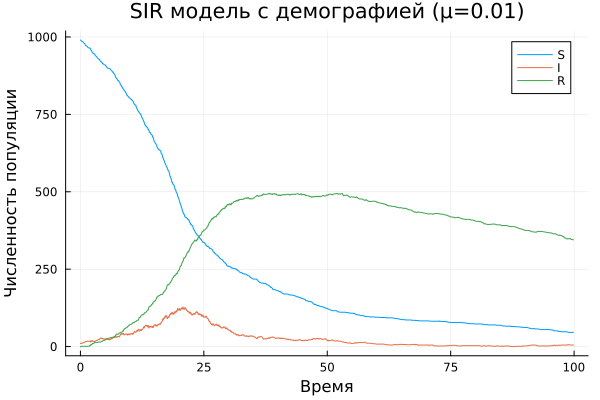
\includegraphics[width=0.7\textwidth,height=\textheight]{image/sir_with_demography.png}

}

\caption{\label{fig-003}добавление возможности смерти и рождения}

\end{figure}%

\textbf{Ниже приведен код, результаты расчетов и графики для кода в
файле scripts/sir\_demographic.qmd}

\section{Модель SIR}\label{ux43cux43eux434ux435ux43bux44c-sir-2}

Модель создается, процессы активируются, и запуск выполняется. Результат
преобразуется во фрейм данных. График с кривыми S, I, R создается и
сохраняется

\begin{Shaded}
\begin{Highlighting}[]
\ImportTok{using} \BuiltInTok{DrWatson}
\PreprocessorTok{@quickactivate} \StringTok{"project"}

\ControlFlowTok{if}\NormalTok{ !}\FunctionTok{isdefined}\NormalTok{(}\BuiltInTok{Main}\NormalTok{, }\OperatorTok{:}\NormalTok{SIRPerson)}
    \FunctionTok{include}\NormalTok{(}\FunctionTok{srcdir}\NormalTok{(}\StringTok{"Sir\_model\_1.jl"}\NormalTok{))}
\ControlFlowTok{end}

\ImportTok{using} \BuiltInTok{StatsPlots}
\FunctionTok{gr}\NormalTok{(fmt}\OperatorTok{=:}\NormalTok{png)}
\end{Highlighting}
\end{Shaded}

\begin{verbatim}
┌ Warning: DrWatson could not find find a project file by recursively checking given `dir` and its parents. Returning `nothing` instead.
│ (given dir: /home/nelianjovu)
└ @ DrWatson ~/.julia/packages/DrWatson/2QF5p/src/project_setup.jl:84
\end{verbatim}

\begin{verbatim}
Plots.GRBackend()
\end{verbatim}

Параметры

\begin{Shaded}
\begin{Highlighting}[]
\NormalTok{p }\OperatorTok{=}\NormalTok{ [}\FloatTok{0.05}\NormalTok{, }\FloatTok{10.0}\NormalTok{, }\FloatTok{0.25}\NormalTok{, }\FloatTok{0.01}\NormalTok{]}
\NormalTok{u0 }\OperatorTok{=}\NormalTok{ [}\FloatTok{990}\NormalTok{, }\FloatTok{10}\NormalTok{, }\FloatTok{0}\NormalTok{]}
\NormalTok{model }\OperatorTok{=} \FunctionTok{MakeSIRModel}\NormalTok{(u0, p)}
\FunctionTok{activate}\NormalTok{(model)}
\FunctionTok{sir\_run}\NormalTok{(model, }\FloatTok{100.0}\NormalTok{)}

\NormalTok{results }\OperatorTok{=} \FunctionTok{out}\NormalTok{(model)}
\end{Highlighting}
\end{Shaded}

\begin{tabular}{r|cccc}
    & t & S & I & R\\
    \hline
    & Float64 & Int64 & Int64 & Int64\\
    \hline
    1 & 0.0 & 990 & 10 & 0 \\
    2 & 0.00934807 & 989 & 11 & 0 \\
    3 & 0.447958 & 988 & 12 & 0 \\
    4 & 0.832778 & 987 & 13 & 0 \\
    5 & 0.926698 & 986 & 14 & 0 \\
    6 & 1.24744 & 985 & 15 & 0 \\
    7 & 1.49851 & 984 & 16 & 0 \\
    8 & 1.54501 & 983 & 17 & 0 \\
    9 & 1.59558 & 982 & 18 & 0 \\
    10 & 1.64916 & 981 & 19 & 0 \\
    11 & 1.6773 & 980 & 20 & 0 \\
    12 & 1.8289 & 979 & 21 & 0 \\
    13 & 1.86758 & 978 & 22 & 0 \\
    14 & 1.9757 & 977 & 23 & 0 \\
    15 & 1.99248 & 976 & 24 & 0 \\
    16 & 2.0526 & 975 & 25 & 0 \\
    17 & 2.11483 & 974 & 26 & 0 \\
    18 & 2.17464 & 973 & 27 & 0 \\
    19 & 2.18082 & 972 & 28 & 0 \\
    20 & 2.21973 & 971 & 29 & 0 \\
    21 & 2.23986 & 970 & 30 & 0 \\
    22 & 2.25402 & 969 & 31 & 0 \\
    23 & 2.39795 & 968 & 32 & 0 \\
    24 & 2.4003 & 967 & 33 & 0 \\
    25 & 2.41576 & 966 & 34 & 0 \\
    26 & 2.49732 & 965 & 35 & 0 \\
    27 & 2.50687 & 964 & 36 & 0 \\
    28 & 2.5274 & 963 & 37 & 0 \\
    29 & 2.57474 & 962 & 38 & 0 \\
    30 & 2.61118 & 961 & 39 & 0 \\
    $\dots$ & $\dots$ & $\dots$ & $\dots$ & $\dots$ \\
\end{tabular}

Визуализация

\begin{Shaded}
\begin{Highlighting}[]
\FunctionTok{plot}\NormalTok{(results.t, [results.S results.I results.R],}
\NormalTok{     label}\OperatorTok{=}\NormalTok{[}\StringTok{"S"} \StringTok{"I"} \StringTok{"R"}\NormalTok{],}
\NormalTok{     xlabel}\OperatorTok{=}\StringTok{"Время"}\NormalTok{, ylabel}\OperatorTok{=}\StringTok{"Численность популяции"}\NormalTok{,}
\NormalTok{     title}\OperatorTok{=}\StringTok{"SIR модель с демографией (μ=}\SpecialCharTok{$}\NormalTok{(p[}\FloatTok{4}\NormalTok{])}\StringTok{)"}\NormalTok{)}
\FunctionTok{savefig}\NormalTok{(}\FunctionTok{plotsdir}\NormalTok{(}\StringTok{"sir\_with\_demography.png"}\NormalTok{))}

\FunctionTok{println}\NormalTok{(}\StringTok{"Готово! μ = "}\NormalTok{, p[}\FloatTok{4}\NormalTok{])}
\end{Highlighting}
\end{Shaded}

\begin{verbatim}
Готово! μ = 0.01
\end{verbatim}

\section{8.
Вакцинация}\label{ux432ux430ux43aux446ux438ux43dux430ux446ux438ux44f}

Я внедряю стратегию вакцинации(рис.15)

\begin{figure}

\centering{


\includegraphics[width=0.7\textwidth,height=\textheight]{image/pic15.png}

}

\caption{\label{fig-003}Вакцинация}

\end{figure}%

На графике мы видим, что в определенный момент времени некоторые из
восприимчивых мгновенно переносят R. Для предотвращения эпидемии
необходимо вакцинировать около 50\% населения(рис.16)

\begin{figure}

\centering{

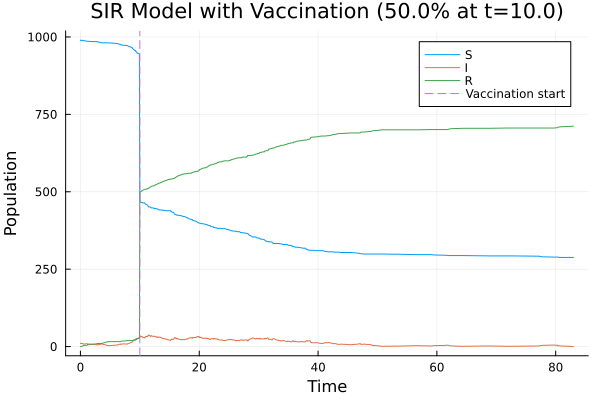
\includegraphics[width=0.7\textwidth,height=\textheight]{image/sir_des_vaccination.png}

}

\caption{\label{fig-016}График вакцинации}

\end{figure}%

\section{9. Модель SEIR}\label{ux43cux43eux434ux435ux43bux44c-seir}

Разница между sir и seir в том, что для sir это восприимчивость -
заражение - выздоровление. Как только вы заразитесь, вы можете заразить
других. В модели seir есть дополнительный этап, который заключается в e
- воздействии, в этом случае, как только вы подвергаетесь воздействию,
требуется время, чтобы вы заразились и были восстановлены.

Я ввожу период ожидания (статус :E)(рис.17)

\begin{figure}

\centering{


\includegraphics[width=0.7\textwidth,height=\textheight]{image/pic16.png}

}

\caption{\label{fig-016}Модель SEIR}

\end{figure}%

При тех же параметрах, что и в модели sir, болезнь распространяется
гораздо медленнее, и в модели seir эпидемии практически
отсутствуют.(рис.18)

\begin{figure}

\centering{

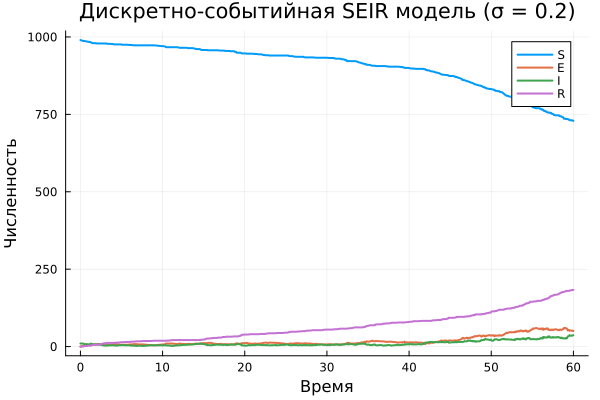
\includegraphics[width=0.7\textwidth,height=\textheight]{image/seir_des.png}

}

\caption{\label{fig-016}График модели SEIR}

\end{figure}%

\textbf{Ниже приведен код, результаты расчетов и графики для кода в
файле scripts/seir.qmd}

Пример использования модели SEIR

\begin{Shaded}
\begin{Highlighting}[]
\ImportTok{using} \BuiltInTok{DrWatson}
\PreprocessorTok{@quickactivate} \StringTok{"project"}
\FunctionTok{include}\NormalTok{(}\FunctionTok{srcdir}\NormalTok{(}\StringTok{"Seir.jl"}\NormalTok{))}
\ImportTok{using} \BuiltInTok{Random}\NormalTok{, }\BuiltInTok{StatsPlots}\NormalTok{, }\BuiltInTok{BenchmarkTools}\NormalTok{, }\BuiltInTok{CSV}\NormalTok{, }\BuiltInTok{Dates}
\FunctionTok{gr}\NormalTok{(fmt}\OperatorTok{=:}\NormalTok{png)}
\end{Highlighting}
\end{Shaded}

\begin{verbatim}
┌ Warning: DrWatson could not find find a project file by recursively checking given `dir` and its parents. Returning `nothing` instead.
│ (given dir: /home/nelianjovu)
└ @ DrWatson ~/.julia/packages/DrWatson/2QF5p/src/project_setup.jl:84
\end{verbatim}

\begin{verbatim}
Plots.GRBackend()
\end{verbatim}

Параметры модели SEIR

\begin{Shaded}
\begin{Highlighting}[]
\NormalTok{tmax }\OperatorTok{=} \FloatTok{60.0}
\NormalTok{u0 }\OperatorTok{=}\NormalTok{ [}\FloatTok{990}\NormalTok{, }\FloatTok{0}\NormalTok{, }\FloatTok{10}\NormalTok{, }\FloatTok{0}\NormalTok{]  }\CommentTok{\# S, E, I, R}
\NormalTok{p }\OperatorTok{=}\NormalTok{ [}\FloatTok{0.05}\NormalTok{, }\FloatTok{10.0}\NormalTok{, }\FloatTok{0.25}\NormalTok{]  }\CommentTok{\# β, c, γ}
\NormalTok{σ }\OperatorTok{=} \FloatTok{0.2}  \CommentTok{\# Скорость перехода из E в I (1/средняя длительность латентного периода)}

\BuiltInTok{Random}\NormalTok{.}\FunctionTok{seed!}\NormalTok{(}\FloatTok{1234}\NormalTok{)}
\end{Highlighting}
\end{Shaded}

\begin{verbatim}
TaskLocalRNG()
\end{verbatim}

Запуск SEIR модели

\begin{Shaded}
\begin{Highlighting}[]
\NormalTok{seir\_model }\OperatorTok{=} \FunctionTok{MakeSEIRModel}\NormalTok{(u0, p, σ)}
\FunctionTok{activate\_seir}\NormalTok{(seir\_model)}
\FunctionTok{seir\_run}\NormalTok{(seir\_model, tmax)}
\NormalTok{data\_seir }\OperatorTok{=} \FunctionTok{out\_seir}\NormalTok{(seir\_model)}
\end{Highlighting}
\end{Shaded}

\begin{tabular}{r|ccccc}
    & t & S & E & I & R\\
    \hline
    & Float64 & Int64 & Int64 & Int64 & Int64\\
    \hline
    1 & 0.0 & 990 & 0 & 10 & 0 \\
    2 & 0.110851 & 989 & 1 & 10 & 0 \\
    3 & 0.24955 & 988 & 2 & 10 & 0 \\
    4 & 0.315197 & 987 & 3 & 10 & 0 \\
    5 & 0.418738 & 987 & 3 & 9 & 1 \\
    6 & 0.457041 & 987 & 3 & 8 & 2 \\
    7 & 0.658997 & 986 & 4 & 8 & 2 \\
    8 & 0.812194 & 985 & 5 & 8 & 2 \\
    9 & 0.913646 & 985 & 5 & 7 & 3 \\
    10 & 1.00373 & 984 & 6 & 7 & 3 \\
    11 & 1.16735 & 984 & 5 & 8 & 3 \\
    12 & 1.18218 & 983 & 6 & 8 & 3 \\
    13 & 1.2699 & 983 & 5 & 9 & 3 \\
    14 & 1.27274 & 983 & 4 & 10 & 3 \\
    15 & 1.28548 & 982 & 5 & 10 & 3 \\
    16 & 1.30828 & 982 & 5 & 9 & 4 \\
    17 & 1.31811 & 982 & 5 & 8 & 5 \\
    18 & 1.38263 & 981 & 6 & 8 & 5 \\
    19 & 1.45015 & 980 & 7 & 8 & 5 \\
    20 & 1.71622 & 980 & 7 & 7 & 6 \\
    21 & 2.07612 & 979 & 8 & 7 & 6 \\
    22 & 2.52487 & 979 & 8 & 6 & 7 \\
    23 & 2.56655 & 979 & 8 & 5 & 8 \\
    24 & 2.5969 & 979 & 7 & 6 & 8 \\
    25 & 2.68616 & 979 & 7 & 5 & 9 \\
    26 & 2.7201 & 979 & 7 & 4 & 10 \\
    27 & 3.07698 & 979 & 7 & 3 & 11 \\
    28 & 3.14162 & 979 & 6 & 4 & 11 \\
    29 & 3.23597 & 978 & 7 & 4 & 11 \\
    30 & 3.25924 & 978 & 7 & 3 & 12 \\
    $\dots$ & $\dots$ & $\dots$ & $\dots$ & $\dots$ & $\dots$ \\
\end{tabular}

Визуализация

\begin{Shaded}
\begin{Highlighting}[]
\NormalTok{plot1 }\OperatorTok{=} \PreprocessorTok{@df}\NormalTok{ data\_seir }\FunctionTok{plot}\NormalTok{(}
    \OperatorTok{:}\NormalTok{t,}
\NormalTok{    [}\OperatorTok{:}\NormalTok{S }\OperatorTok{:}\NormalTok{E }\OperatorTok{:}\NormalTok{I }\OperatorTok{:}\NormalTok{R],}
\NormalTok{    labels }\OperatorTok{=}\NormalTok{ [}\StringTok{"S"} \StringTok{"E"} \StringTok{"I"} \StringTok{"R"}\NormalTok{],}
\NormalTok{    xlab }\OperatorTok{=} \StringTok{"Время"}\NormalTok{,}
\NormalTok{    ylab }\OperatorTok{=} \StringTok{"Численность"}\NormalTok{,}
\NormalTok{    title }\OperatorTok{=} \StringTok{"Дискретно{-}событийная SEIR модель (σ = }\SpecialCharTok{$}\StringTok{σ)",}
\StringTok{    }\NormalTok{linewidth}\StringTok{ = 2,}
\NormalTok{)}
\FunctionTok{savefig}\NormalTok{(}\FunctionTok{plotsdir}\NormalTok{(}\StringTok{"seir\_des.png"}\NormalTok{))}
\FunctionTok{display}\NormalTok{(plot1)}
\end{Highlighting}
\end{Shaded}

\includesvg{simmod-lab08-report (Нджову Нелиа)_files/figure-pdf/cell-17-output-1.svg}

\chapter{Выводы}\label{ux432ux44bux432ux43eux434ux44b}

В этой лабораторной работе, я изучила дискретно-событийный подход к
моделированию на примере классической модели распространения инфекции
SIR, как реализовать стохастическую дискретно-событийную модель в Julia
и как анализировать влияние параметров, сравнивать их со стохастическими
и детерминированными версиями, оценивать производительность и
модифицировать систему

\chapter*{Список
литературы}\label{ux441ux43fux438ux441ux43eux43a-ux43bux438ux442ux435ux440ux430ux442ux443ux440ux44b}
\addcontentsline{toc}{chapter}{Список литературы}

\begin{enumerate}
\def\labelenumi{\arabic{enumi}.}
\tightlist
\item
  Кулябов Д.С. simulation-modeling-lab.pdf. 8 Реализация основных
  моделей в дискретно-сщбытийном подходе. {[}Электронный ресурс{]}
\end{enumerate}


\printbibliography


\end{document}
